\documentclass[12pt]{article}
\usepackage[pdftex]{graphicx}
\usepackage{multicol}
\usepackage{amssymb}
\title{Geometric Evolution on Computationally Abstract Manifolds}
\pagestyle{plain}
\author{Alex Henniges \\ Thomas Williams \\ Mitch Wilson \\ \\ University of Arizona Undergraduate Research Program\\
Supervisor: Dr. David Glickenstein\\
}
\date{June 30, 2008}
\begin{document}
\maketitle	

\newpage
\section{Introduction}
\maketitle
\subsection{Purpose}
\maketitle

Over the course of the summer, we aim to develop code that will allow us to construct these triangulations and be able to perform Ricci flow on these manifolds. As we progress, we aim to dig deeper into the subject, investigating new ideas and applications as they arise. Our initial plan of action is to

\subsection{Outline of paper}
\maketitle

The remainder of this paper is arranged as such:
\begin{itemize}
\item Triangulations- definitions, concepts, and properties
\item Combinatorial Ricci flow- history, applications, and equations. 
\item Progamming/Code- our methods for solving these problems
\item Results- Interpretation, specfic cases, and convergence analysis
\item Future work- Potential projects for the weeks ahead
\end{itemize}

\section{Triangulations}
\maketitle
\subsection{Introduction}
\maketitle

Suppose you are asked to make a sphere, but are only given a small number of edges, vertices, or faces to work with. What do you do? In geometry, a common question asked is how to make representations of complex shapes with as little stuff as possible. In fact, you are probably already familiar with the most basic representation of a sphere- a tetrahedron. Using only four vertices, six edges, and four faces, the tetrahedron is able to give us an approximation to a sphere. Similarly, three vertices (a triangle) can be used to approximate a circle in two dimesnions. Naturally, if we add more vertices, we are able to better illustrate our shapes. \newline
  
   \noindent Of course, spheres aren't the only things geometers care about. Another shape of interest is known as the torus. It looks like a donut. It turns out that you can make a visualization of this object using only 7 vertices \cite{lutzmanifold}. With more vertices the shape becomes better curved and reminiscent of breakfast. Mmm, torus. It is also possible to add ''handles'' to any shape, resulting in the addition of another torus. There are also various other shapes which can be represented with varying numbers of vertices, like Klein bottles and cross-caps.\cite{WolfMath} has more information on these fascinating shapes.\newline
   
   \noindent Like in modern video games and Hollywood movies, we can generate various shapes of many different sizes using polygons that mold to form the special effect. For these and all shapes, we will focus on building them solely out of triangles. Since any regular polygon can be broken up into smaller triangles, we can essentially represent any shape with enough vertices. We define a shape as $triangulizable$ if we can connect all triangles in a particular fashion such that they create a closed 3-dimenional shape.\newline
  
\begin{figure}
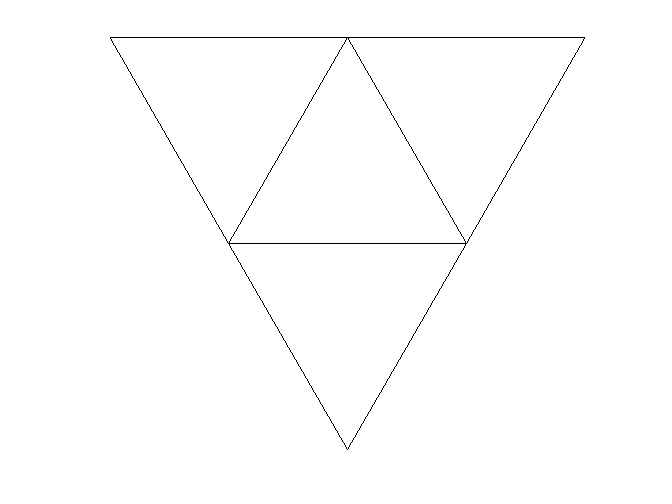
\includegraphics[scale = 0.5]{flattetrahedron.png}
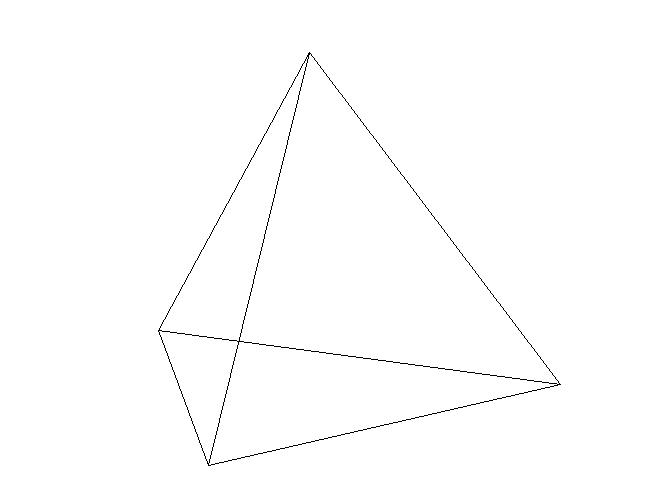
\includegraphics[scale = 0.3]{tetrahedron.jpg}
\caption{An example of triangulation. A triangle can be folded up into a tetrahedron.}
\end{figure}

\noindent An issue arises regarding the uniqueness of these triangulations. There are over 28 $trillion$ ways to triangulate a sphere using only 23 vertices. It is currently unknown how many ways a single torus can be made using that number of vertices (to us, at least). However, all toruses do share something very peculiar, as do all sphere configurations. The Euler characteristic, $\chi$, is a value associated with three dimensional shapes. It is defined as $\displaystyle\chi = V - E + F$, where $V,$ $E,$ and $F$ are the number of vertices, edges, and faces a given manifold has. Certain shapes have the same $\chi$ value. For example, any torus has $\chi = 0$, and any representation of a sphere has $\chi = 2.$ Table \ref{EuChar} has listings for many common shapes. \newline

\subsection{Circle packing}
\maketitle

\noindent While we can indicate how these different vertices are connected to each other, there is still an issue regarding the lengths of these edges. There are an infinite number of possible edge length configurations just as there are an infinite number of possible triangles. We introduce to the reader a method known as circle packing to quantify edge lengths. In circle packing, the shapes in question can be constructed using circles of the same dimension on each of the vertices. Circles can be used to make the sides of a triangle; spheres can be used to make the edges of a tetahedron. These circles are mutually tangent to each other, and two radii make up one edge. Thus, the length is simply the sum of the two radii of the adjacent vertices $l_{ij} = r_i + r_j$.
  
\begin{figure}
\begin{center}
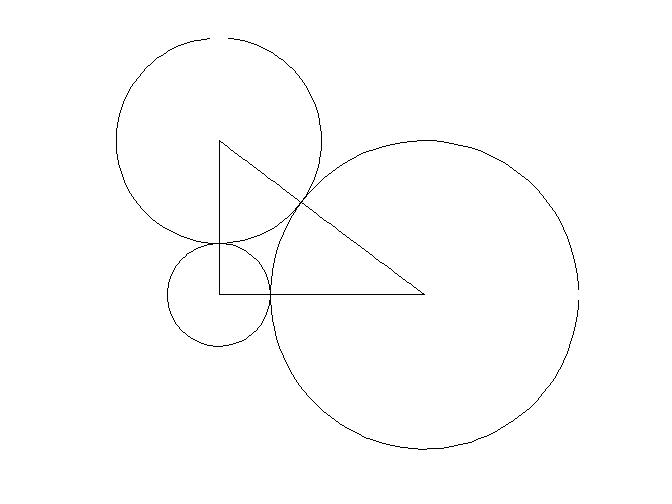
\includegraphics[scale = 0.3]{righttriangulation.jpg}
\end{center}
\caption{An example of circle packing. Three mutually tangent circes forming the perimeter of a triangle.}
\end{figure}

\begin{table}
\begin{tabular}{ccccc}
Name  &	Vertices, V &	Edges, E & Faces, F &	$\chi, V - E + F$\\
\hline 
Tetrahedron &	4 &	6 &	4 &	2\\
Hexahedron or cube &	8 &	12 &	6 &	2\\
Octahedron 	&	6 &	12 &	8 & 2\\
Dodecahedron 	&	20 &	30 &	12 &	2\\
Icosahedron &	12 & 30 & 20 &	2\\
Torus & 9 & 27 & 18 & 0\\
Double torus & 10 & 36 & 24 & -2
\end{tabular}
\caption{Listings of vertices, edges, and faces for some common shapes \cite{wiki}}
\label{EuChar}
\end{table}

\begin{figure}
\centering
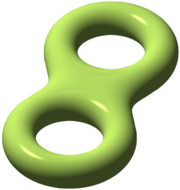
\includegraphics[scale = 2.0]{180px-Double_torus_illustration.png}
\caption{This is a double torus. It has $\chi$ = -2.} %\hrulefill
\label{test}
\end{figure}

\subsection{Duals}
\maketitle

Every triangle that is capable of being circle-packed has a circle that is internally tangent to all three edges. It is known that this $incircle$ is perpendicular to each edge and has a radius $\displaystyle r = \sqrt{\frac{(s-a)(s-b)(s-c)}{s}}$ where $s$ is the semi-perimenter of the triangle, and $a, b, $and $c$ are the side lengths. Let us rewrite this in terms of the vertex weights, since we are using circle packing. Thus, a side length is simply the sum of two vertex radii. We can then simplify this equation to $\displaystyle r = \sqrt{\frac{r_i r_j r_k}{r_i + r_j + r_k}}$, with $i, j $and $k$ being the vertices of a triangle. This can be repated for multiple triangles. As a plus, all these incircles are mutually tangent. We can define a dual edge $\star e$ as the sum of the radii of the incircles with that side in question. $\star e = r_{in1} + r_{in2}$. See Figure~\ref{fig:dual} for an illustration of a dual edge.\newline

\begin{figure}
\centering
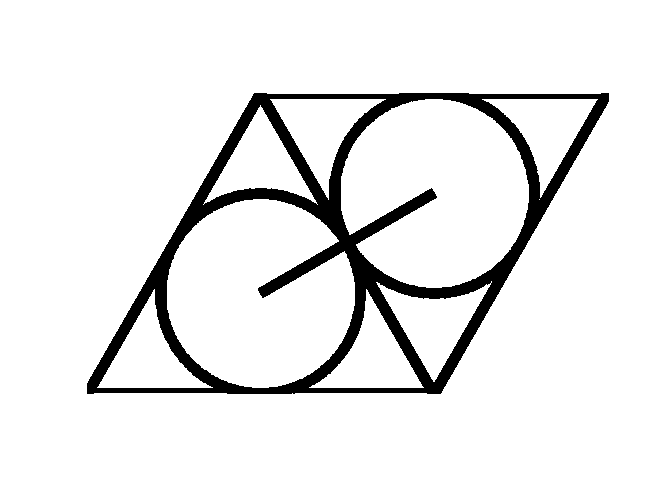
\includegraphics[scale = 0.4]{dual.png}
\caption{A dual to an edge}
\label{fig:dual}
\end{figure}

\noindent With enough dual edges, we can obtain a polygon surrounding a vertex. The area of the region formed by these duals is called the dual area, evaluated by $$\star A_i = r_i\sum{\frac{\star e_i}{2}} = r_i\sum{r_{\mbox{inscribed}}}$$

\noindent The dual length and dual area have some interesting properties that we hope to investigate. David Glickenstein examines these and more in \cite{Dave}.  

\section{Ricci flow}
\subsection{Background}

Introduced by Richard Hamilton in 1982, Ricci flow, named in honor of Gregorio Ricci-Curbastro \cite{RicciBkgd}, has since made large impacts in the world of geometry and topology. It is often described as a heat equation. Imagine a room where a fireplace sits in one corner and a window is open on the other side. The heat will diffuse through the room until the temperature is the same everywhere. With Ricci flow, the same occurs with the curvature. Under Ricci flow, a geometric object that is distorted and uneven will morph and change as necessary so that all curvatures are even.\newline

\noindent But the biggest consequence of Ricci flow was not to become apparent until early after the turn of the millenium, when Grigori Perelman presented three papers providing the proof to the Poincar\'{e} Conjecture. The Poincar\'{e} Conjecture, proposed in 1904, proved to be particularly difficult to prove, and was given the honor of one of seven millenium puzzles by the Clay Matehmatics Institute. It was Ricci flow that turned out to be the cornerstone for the proof. In addition, its relation to the heat equation may open new doors for work in fluid dynamics and even in the theory of general relativity \cite{RicciBkgd}. 


\subsection{Definition}

Just because we have a triangulation and that it is circle packed does not mean that it is already compact and organized. Vertices can be too large or too small, and the end shape can be somewhat repulsive. We would like to have a way to make these radii as uniform as possible while keeping the original shape intact. We introduce the equation for combinatorial Ricci flow, which allows an individual radius to change over time. In Euclidean space, the differential equation can be written as 
  \begin{equation}
  \label{Riccif}
  \frac{dr_i}{{dt}} = -K_ir_i
  \end{equation}
  
\noindent where $K_i$ is a characteristic called the curvature of a vertex, and $r_i$ is the radius or weight of a vertex $i$. The value of $K_i$ changes with time. Its value is found by determining the angles of all triangles containing vertex $i$. Using side lengths (or radii) we can determine the angle using the law of cosines. For a triangle with lengths $a, b$ and $c,$ the angle opposite side $c$ is:
  
  \begin{eqnarray*}
  \angle C = \arccos\frac{a^2 + b^2 - c^2}{2ab}
  \end{eqnarray*} 
  
\noindent with similar formulas for the other angles. We take the sum of all angles associated with a vertex $i$ and define the curvature $K_i$ as:

  \begin{equation}
  K_i = 2\pi - \sum{\angle i}
  \end{equation}
  
\noindent So since the differential equation depends on a variable whose value changes over time, we cannot solve it so easily.\newline
   
\noindent A potential issue we noted is that based on the equation, more often than not, the lengths of the radii would decrease. Take the example of a simple tetrahedron with all sides of equal length, we find that the curvature of each vertex always equals $\pi$. Thus in solving the differential equation computationally we would decrease each vertex by the same amount, but the curvature of each vertex would still remain $\pi$. The radii would continue to decrease until they approach zero length. We then have to address that issue since computers don't like working with numbers near zero, as in the denominator of the arccosine function. Weird, unwanted stuff might happen. Let us introduce the ability to resize the length of each radius by a scalar, $\alpha$. We denote each scaled length by $\tilde{r_i}$ and equate as
 
 \begin{equation}
 \tilde{r_i} = \alpha r_i
 \end{equation} 
 
\noindent Thus in plugging in to the differential equation we get
 
 \begin{eqnarray}
 \label{ref1}
 \frac{d\tilde{r_i}}{dt} &=& \frac{d(\alpha r_i)}{dt} = \alpha \frac{dr_i}{dt} + r_i\frac{d\alpha}{dt}\nonumber\\
 &=& -\alpha K_ir_i + \frac{\tilde{r_i}}{\alpha}\frac{d\alpha}{dt} \nonumber \\
 &=& -\tilde{K_i}\tilde{r_i} + \frac{\tilde{r_i}}{\alpha}\frac{d\alpha}{dt}
 \end{eqnarray}
 
\noindent Since we are scaling all sides by the same factor, this does not effect the curvature of the surface, so $\tilde{K_i} = K_i$. It also turns out that $$\displaystyle \frac{1}{\alpha} \frac{d\alpha}{dt} = \frac{d(\mbox{log}~\alpha)}{dt}$$ 
 In order to find an appropriate value for $\alpha$ we decided to use the following criteria:
 
\begin{equation}
\label{eqprod}
\prod{\tilde{r_i}(t)} = \prod{\alpha r_i(t)} = C\mbox{, a constant}
\end{equation}

\noindent This can be used to prevent radii from decreasing to zero. It turns out if you take the derivative of ($\ref{eqprod}$) with respect to time you find that 
 
\begin{equation}
\label{proof1}
\frac{d(\mbox{log}~\alpha)}{dt} = \frac{\mbox{sum of all curvatures}}{\mbox{number of vertices}} = \overline{K}, \mbox{average curvature}
\end{equation}
 
\noindent It turns out that $\overline{K}$ is constant for any iteration of our triangulation and is equal to $\displaystyle\frac{2\pi\chi}{|V|}$, where $|V|$ is the number of vertices and $\chi$ is the Euler characteristic. This is noted in \cite{chowluo}. Plugging this back into ($\ref{ref1}$) we determine that

\begin{equation}
\frac{d\tilde{r_i}}{dt} = -\tilde{K_i}\tilde{r_i} + \overline{K}\tilde{r_i} = (\overline{K} - K_i)\tilde{r_i}
\end{equation}

\noindent However, since everything is now a function of $\tilde{r_i}$ and not $\alpha$, we can treat $\alpha$ as a constant and thus $\displaystyle\frac{d\alpha}{dt} = 0$. Therefore, we can easily plug $\tilde{r_i} = \alpha r_i$ back in to the differential equation, so we end up with:

\begin{eqnarray}
\label{Riccin}
\frac{d\tilde{r_i}}{dt} &=& (\overline{K} - K_i)\tilde{r_i} \nonumber \\
\alpha\frac{dr_i}{dt} &=& (\overline{K} - K_i)\alpha r_i \nonumber \\
\frac{dr_i}{dt} &=& (\overline{K} - K_i)r_i
\end{eqnarray}

\noindent This is known as normalized Ricci flow, as discussed in \cite{chowluo}. In the case of our basic tetrahedron from earlier, the radii would not change after each iteration as $\overline{K} = K_i = \pi$ for each vertex and thus $\displaystyle\frac{dr_i}{dt} = 0$. With its roots in differential geometry, Ricci flow has become a popular topic in mathematics, finding uses and applications in many different fields. It even helped solve one of the Millenium Puzzles, valued at \$1,000,000, in 2003. \cite{wikipoin}  

\subsection{Expectations}

With regards to our program, Ricci flow over 2-manifold Euclidean surfaces will be important as a good way to test the code. Cases like the tetrahedron can be calculated by hand so it will be useful to test our results against them. For example, we expect that the Tetrahedron under (\ref{Riccif}) will have all weights converge to zero. Whereas under (\ref{Riccin}) the weights are expected to converge to positive constants.\newline

\noindent
There are other expectations beyond those we can calculate by hand.

\section{Program/Code}
\subsection{Structure}

When beginning the creation of the program, the structure design was critical. Not only would it help dictate the direction of the project over the course of its lifespan, but the design decisions would affect the speed and efficiency of all added functionality. It was agreed that system would have to hold the different simplices and that they would be referencing each other. This part of the program would need to be structured in a way that was quick and easy to move from one simplex to another. As seen in figu.\ref{triUML}, all simplices are assumed to have lists of references to other simplices, what we call local simplices, broken down by dimension. So for the two-dimensional case, each simplex has lists of local vertices, local edges, and local faces, as shown in Table~\ref{geomat}.\newline

  \begin{table}[b]
  \begin{center}
  \begin{tabular}{|c|c|c|}
  \hline
  Vertices & Edges & Faces\\
  \hline
  adjacent vertices & component vertices & component vertices\\
  constructed edges & adjacent edges & component edges\\
  constructed faces & construced faces & adjacent faces\\
  \hline
  \end{tabular}
  \end{center}
  \caption{A layout of how data is organized}
  \label{geomat}
  \end{table}
  
\noindent The lists are vectors of integers. The vector, provided in the C++ library, was chosen so that the list can dynamically change in size. The integers are a decision based on both speed and size. Instead of, for example, a vertex having a list of actual edges ($\overline{AB}, \overline{CF},$ etc.) or pointers to edges, the vertex has a list of integers representing the edges. The actual edges are then obtained through the $Triangulation$ class, which holds maps from integers to simplices. The $Triangulation$ class is made up of static methods and maps and is designed so only one triangulation exists at any time. Because the maps are static, they can be accessed at any time from anywhere in the code without the need to pass pointers through function calls. Vertices also hold a weight, representing the radii from a circle packing on the triangulation. Edges then have a length based on the weights of its two vertices. When a vertex's weight is changed, the local edges to that vertex act as an observer and will update their lengths automatically.\newline

\noindent While we are able to manually construct a few basic triangulations by hand, as we add more vertices that will become ever harder. \cite{lutzmanifold} has millions of known triangulations of varying size. However, the format is different than our setup, so we developed an algorithm to take a given triangulation, saved on its own as a text file, and be able to convert it into the form that we use. We were able to transform this
  
\begin{verbatim}{manifold_lex_d2_n5_o1_g0_#1=[[1,2,3],[1,2,4],[1,3,4],
[2,3,5],[2,4,5],[3,4,5]]}
\end{verbatim}
 
which solely documents the faces, into this:

% Table generated by Excel2LaTeX from sheet 'Sheet1'
\begin{table}
\begin{center}
\begin{tabular}{|r|r|r|}
\hline
 Vertex: 1 &    Edge: 1 &    Face: 1 \\ \hline 

     2 3 4 &        1 2 &     1 2 3  \\

    1 2 4  & 2 3 4 5 7  &     1 2 3  \\

    1 2 3  &       1 2  &     2 3 4  \\ \hline 

 Vertex: 2 &    Edge: 2 &    Face: 2 \\ \hline

   1 3 4 5 &        1 3 &     1 2 4  \\

  1 3 5 7  & 1 3 4 6 8  &     1 4 5  \\

  1 2 4 5  &       1 3  &     1 3 5  \\ \hline 

 			\vdots & \vdots & \vdots \\ \hline 

 Vertex: 5 &    Edge: 9 &    Face: 6 \\ \hline

     2 3 4 &        4 5 &     3 4 5  \\

    7 8 9  & 4 5 6 7 8  &     6 8 9  \\

     4 5 6 &       5 6  &     3 4 5  \\
\hline
\end{tabular}
\end{center}
\caption{Conversion of format from \cite{lutzmanifold} to ours.}
\end{table}  

\noindent which allows us to keep track of every vertex, edge, and face.

\subsection{calcFlow}

\noindent The function $calcFlow$ runs a Ricci flow over the triangulation and records the data in a file. The algorithm for the ODE, provided by J-P Moreau, employs a Runge-Kutta method \cite{JPM}. First, the file name for the data to be written in is provided. Then, a $dt$ is given by the user that represents the time step for the system. The next parameter is a pointer to an array of initial weights to use. This is followed by the number of steps to calculated and record. Lastly, a boolean is provided, where $true$ indicates that the adjusted differential equations that are scaled to a constant, equation (\ref{Riccin}) should be used. Otherwise, the standard equation (\ref{Riccif}) is employed. Printed to the file is each step with every vertex and its weight and curvature at that moment. At the end of each step, the net curvature is printed, as shown below. \newline 
\begin{multicols}{2}
\begin{tabular}{l|l|l}
\hline
Step 1   & Weight &  Curv\\
Vertex 1:& 6.000 & 0.7442\\
Vertex 2: &3.000 & -1.122\\
Vertex 3:& 3.000 & -1.373\\
Vertex 4:& 8.000 & 1.813\\
Vertex 5: &6.000 & 1.227\\
Vertex 6: &2.000 & -3.046\\
Vertex 7: &4.000 & -0.3045\\
Vertex 8: &8.000 & 1.989\\
Vertex 9: &5.000 & 0.07239\\ \hline
\end{tabular} Net Curv: 0.0000 

\begin{tabular}{l|l|l}
\hline
Step 50 &  Weight &  Curv\\
Vertex 1:& 4.557 & 0.008509\\
Vertex 2: &4.530 & -0.01185\\
Vertex 3: &4.534 & -0.009091\\
Vertex 4:& 4.563 & 0.01268\\
Vertex 5:& 4.550 & 0.002772\\
Vertex 6: &4.527 & -0.01455\\
Vertex 7: &4.541 & -0.003563\\
Vertex 8: &4.559 & 0.01018\\
Vertex 9: &4.553 & 0.004906\\ \hline
\end{tabular}
Net Curv: 0.0000
\end{multicols}

\noindent After the initial design of $calcFlow$, tests were run to determine its speed. The time it took to run was directly proportional to the number of steps in the flow. However, it was also proportional to more than the square of the number of vertices of the triangulation. As a result, while a four-vertex triangulation can run a 1000 step flow in three seconds, it would take a twelve-vertex triangulation 43 seconds to run the same flow. After inspecting the speed of the non-adjusted flow in comparison, it became clear that the calculation of net curvature, which remains constant in two-dimensional manifold cases, was being calculated far too often. After being adjusted so that it is calculated just once per step, the speed of the flow is much faster so that a four-vertex system with 1000 steps takes just one second and twelve vertices is much improved with a time of only four seconds. As expected, the net curvatures of our trials remained constant, ensuring that our program was running as we expected it to.\newline

\begin{figure}
\includegraphics[scale = 0.5]{triangulationUML.png}
\caption{A layout of commands and how they are connected.}
\label{triUML}
\end{figure}

\subsection{Morphs}

\subsubsection{Flips}

There may be times where we want to change a given triangulation by a small amount. Rather than start from scratch, we can perform flips. $Flips$ are a technique which change the topology of a surface by a small degree. There are three basic types:

\begin{itemize}
\item 1-3 flip \newline
Here we take a triangle and turn it into three triangles. In other words, we add a vertex to a triangulation and connect it to the three vertices of the triangle it is inside. If we performed this on each face of a tetrahedron, we would result in a dodecahedron, a solid with 12 faces, three from each original face of the tetrahedron. After running this through $calcFlow$, all the new vertices form 45-45-90 degree isosocles right triangles with the old vertices constructing the hypoteneuses. 
\item 2-2 flip \newline
In this flip we take an edge that is part of two faces, and switch the vertices. See figure~\ref{fig:flip}. 
\item 3-1 flip \newline
Here we do the opposiste of a 1-3 flip. We take a vertex that is connected to three other vertices and remove it entirely. This move is more restrictive than the others since not every vertex is connected to exactly three vertices. 
\end{itemize}
\begin{figure}
\centering
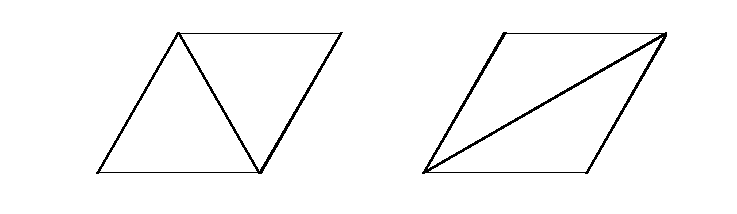
\includegraphics[scale = 1.0]{Flip.png}
\caption{An example of a flip.}
\label{fig:flip}
\end{figure}
  
\begin{figure}
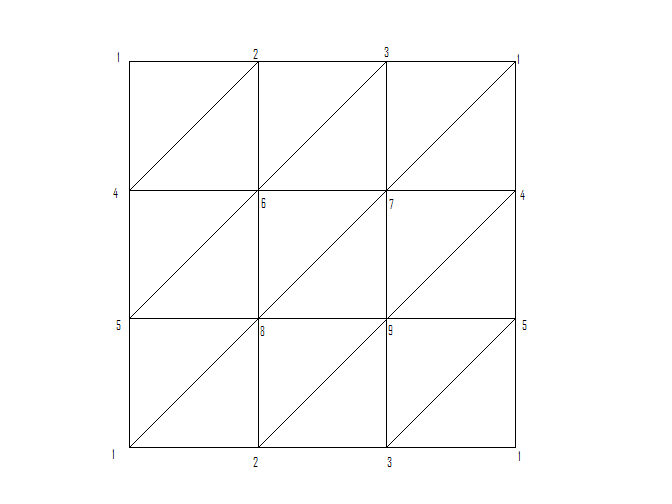
\includegraphics[scale = 0.5]{torus2.png}
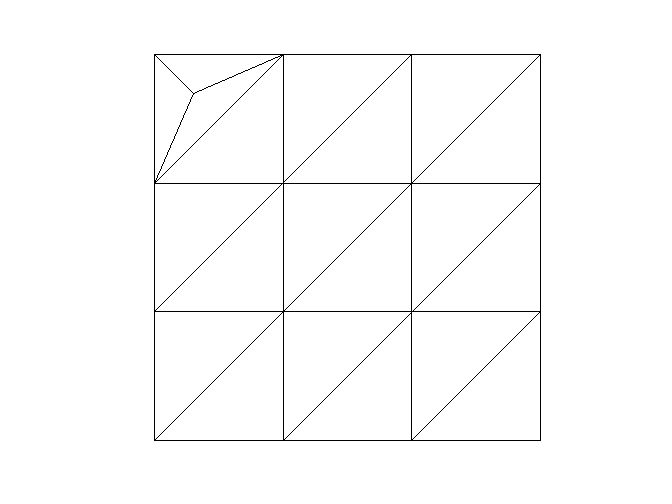
\includegraphics[scale = 0.5]{torus2addvertex.png}
\caption{A triangulation of the torus, and the addition of a new vertex.}
\label{torusaddv}
\end{figure}

\subsubsection{Adding handles and leaves}
We can add a torus handle to a triangulation. This instantly reduces the $\chi$ value of the surface by 2.\newline

Another shape we have been looking into is called the double triangle. In essence, a double triangle is made of two triangles with the same three vertices. It can though of as folding one triangle on top of another. We can add these, which can be called leaves, to a triangulation and see how things vary with their presence. However, upon adding a double triangle, we have uncertainty regarding our definiton of a triangulation. 

\section{Results}

\subsection{Flows}

The program for the Ricci flow was tested by beginning with the most simple cases, and then explored as many different possibilities as we could conceive of to try to find any anomalies. The first test was the tetrahedron. In the standard equation, it is easily shown that all weights approach zero exponentially fast. In the normalized equation, and the equation that is used in the rest of the testing, the tetrahedron's weights approach a single positive number, the fourth root of the ``area'' of the tetrahedron, so that the area remains constant. In addition, all the curvatures converged to the same value, in this case ($\pi$) so that the net curvature is ($4\pi$). Results were similar for the other platonic solids.\newline

\noindent The next test was the torus with the standard nine-vertex triangulation. Again all the weights approached the same positive number to maintain constant area. As expected, the curvatures all went to zero while the total curvature remained zero throughout. Further simple tests included triangulations of larger genus, and in all cases the total curvature remained at the constant multiple of ($\pi$) that was expected and the ``area'' was also constant. In addition, there does not appear to be any further affect from the initial weights then determining the area of the triangulation. It is not clear from any of the tests we ran that having extremes amongst the initial weights causes a different end result.\newline

\noindent In each case all vertices converged to the same curvature. This was not always the situation for the weights, as in many triangulations there would be several final weights. It became clear that this would occur when vertices had different degrees. In fact, we feel fairly certain that there might be a formula relating the area of a weighted triangulation and the degree of a vertex to that vertex's final weight. In most of the examples we tried, when two vertices had the same degree, they had the same final weight, but this is not always the case. One such example is adding three vertices to one face of the tetrahedron. As seen in Table (\ref{tab:Vres}) vertices 4, 5, and 6 all have degree four. Yet vertex 5 has a greater final weight than the other two. The only explanation we could find with some merit is that the local vertices of 5 are different in degree from those of 4 and 6. That is, the degrees of the local vertices of 5 are never less than four, while vertices 4 and 6 each have a local vertex with degree 3.


% Table generated by Excel2LaTeX from sheet 'Sheet1'
%\begin{table}
%\begin{center}
%\begin{tabular}{|r|r|r|}
%\hline
% \underline{Vertex: 1}           &  Vertex: 5             & Final weights for a random             \\ \hline
%
%2 3 4 5 6 7              &   1 2 4 6             & initial weighted Triangulation            \\
%
%1 2 3 7 10 13              &  7 8 9 12              & Vertex 1: 15.692            \\
%
%1 2 3 5 7 9              &   5 6 7 8              & Vertex 2: 15.692            \\ \hline
%
% Vertex: 2             &  Vertex: 6            & Vertex 3: 6.18421            \\ \hline
%
%1 3 4 5 6 7              &   1 2 5 7             & Vertex 4: 9.6524           \\
%
%1 4 5 8 11 14             & 10 11 12 15              & Vertex 5: 10.6409            \\
%
%1 2 4 6 8 10              &  7 8 9 10              & Vertex 6: 9.6524           \\ \hline
%
% Vertex: 3            &  Vertex: 7            & Vertex 7: 6.18421          \\ \hline
%
%    1 2 4              &     1 2 6              &                      \\
%
%    2 5 6              &  13 14 15              &                       \\
%
%    2 3 4              &    1 9 10              &                      \\
%
% Vertex: 4            &                        &                       \\
%
%  1 2 3 5              &                       &                     \\
%
%  3 4 6 9              &                        &                      \\
%
%  3 4 5 6             &                     &                   \\
%\hline
%\end{tabular}
% Table generated by Excel2LaTeX from sheet 'Sheet1'
\begin{minipage}[b]{0.5\linewidth}

\begin{tabular}{|l|l|}
\hline
 Vertex: 1 &  Vertex: 5 \\
\hline
2 3 4 5 6 7  &   1 2 4 6  \\

1 2 3 7 10 13  &  7 8 9 12  \\

1 2 3 5 7 9  &   5 6 7 8  \\
\hline
 Vertex: 2 &  Vertex: 6 \\
\hline
1 3 4 5 6 7  &   1 2 5 7  \\

1 4 5 8 11 14  & 10 11 12 15  \\

1 2 4 6 8 10  &  7 8 9 10  \\
\hline
 Vertex: 3 &  Vertex: 7 \\
\hline
    1 2 4  &     1 2 6  \\

    2 5 6  &  13 14 15  \\

    2 3 4  &    1 9 10  \\
\hline
 Vertex: 4 &            \\ \hline

  1 2 3 5  &            \\

  3 4 6 9  &            \\

  3 4 5 6  &            \\ 
\hline
%\caption{A complete output of vertices}
\end{tabular}


\end{minipage}
\begin{minipage}[b]{0.5\linewidth}
% Table generated by Excel2LaTeX from sheet 'Sheet1'

\begin{tabular}{|l|}
\hline
Final weights for a random \\

initial weighted Triangulation \\
\hline
Vertex 1: 15.692 \\

Vertex 2: 15.692 \\

Vertex 3: 6.18421 \\

Vertex 4: 9.6524 \\

Vertex 5: 10.6409 \\

Vertex 6: 9.6524 \\

Vertex 7: 6.18421 \\
\hline
\end{tabular}
\label{tab:Vres}
\end{minipage}


\subsubsection{Evaluating expectations}

\subsection{Convergence speeds}

One experiment we performed was measuring convergence speeds of various triangulations. For each triangulation, five flows were run where the weights were random between one and twenty-five. Random weights, while not a perfect solution, was the only viable as it was unclear what set weights could be equal for all triangulations. The dt was held constant at 0.03. For each run, a step number was assigned for when all weights and curvatures had converged to four digits, (the precision shown in a file of the results).  The data collected at times seemed interesting and followed a pattern while other times were inexplicable.\newline

\noindent Beginning with the basic case, the tetrahedron took on average 156.8 steps to converge to four digits and remained fairly consistent through all five trials. Strangely, the octahedron converged faster on all five flows, averaging 138.4 steps. This was made all the stranger by the fact that the icosahedron averaged 198.8 steps. The torus revealed several things about convergences. First, the standard nine vertex torus averaged only 110 steps, suggesting that a torus converges faster than a sphere. When a vertex was added to the torus, it greatly decreased the convergence speed, to 248.8 steps. Compared to the Tetrahedron with an added vertex, 164.2, this was a very large jump. When another vertex was added to the same face as the first, the convergence speed dropped yet again, to an average of 437.6 steps. Yet when this vertex was added to a face not connected to the first, the convergence speed was almost steady at 264.8. And adding a third in the same style caused little increase.\newline

\noindent This seems to suggest that convergence speed is dependent on the number of unique vertices. By unique we mean the properties of the vertex (number of local vertices, convergence weight, etc.). When the vertices were added to separate faces, there remained only three unique vertices. Whereas, adding the two vertices to the same face created five unique vertices. This theory is further supported by a twelve vertex sphere designed so that all vertices are unique. The average convergence was 460 steps, more than twice as long as the icosahedron, which also is a twelve vertex sphere.\newline

\noindent As a final note, the deviation of the initial weights did not have a clear impact on the convergence speed. At some times, it would appear that initial weights with a higher deviation would converge faster, yet at other times it was lower deviation that seemed to lead to faster convergence.

\begin{figure}
\centering
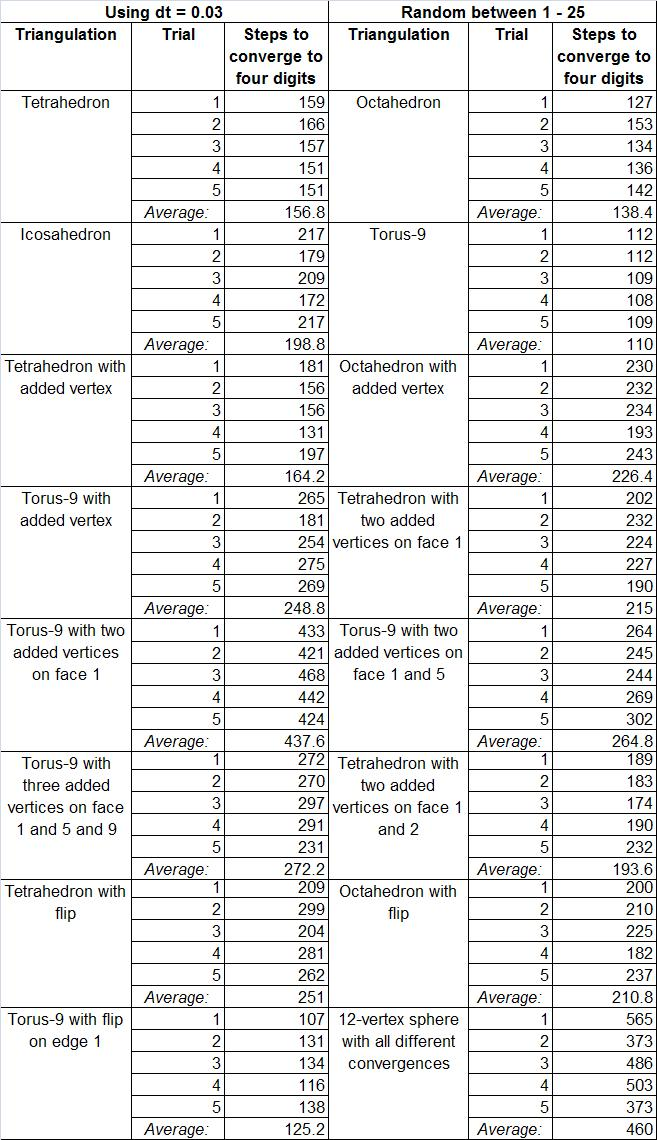
\includegraphics[scale = 0.79]{ConvergenceTable.png}
\caption{Summary of convergence data for varying criterium}
\label{fig:conv}
\end{figure}

\subsection{Specific cases}

\noindent Example: Adding a vertex to a one-holed torus. See figure~\ref{torusaddv}. \newline

\noindent By inserting a vertex within a flat triangulation for a torus, we essentially place a sphere on top of three ofther spheres, and then observe what happens as we run it trough out $calcFlow$ program. We discover that the new vertex gets squeezed in between the other vertices and decreases in size, as if it were never there at all. To counter this, the other vertices grow slightly to maintain Eq.~(\ref{eqprod}). The new vertex lies completely within the void not occupied by the other three triangles. We also ran this test with a 7-vertex torus and obtained similar results. The additional vertex tried to disappear altogether, and even with normalized Ricci flow its weight dropped down to zero, as if it weren't there at all. While this does break our code, we find it very interesting. I wonder if it matters which face you add the vertex to. \newline

\noindent Example: Performing a 2-2 flip on a 12-vertex torus. \newline

\noindent One interesting observation we found was that flips change the asymptotic behavior of some vertices. For Example, in a 12-vertex torus, performing a flip on one edge affected the end radii of many vertices. In fact, their radii was a function of time was not always monotonic! We would occasionally have a vertex change direction before ultimately approaching a limit.\newline 

\noindent Example: two tetrahedra connected at a vertex. It turns out $\chi = $7 Vertices - 12 Edges + 8 Faces = 3, which is not a case we had seen before. In previous cases $\chi$ was an even integer. Starting each vertex with equal weight, we obtained an unexpected result. The center weight becomes very large, and the others become smaller in comparison. We concluded that since the central vertex now had a much lower curvature than the other vertices, it reacted differently to $calcFlow$. One good thing we noted was that the net curvature = $6\pi = 2\pi\chi$, which was a relief.  

\begin{figure}
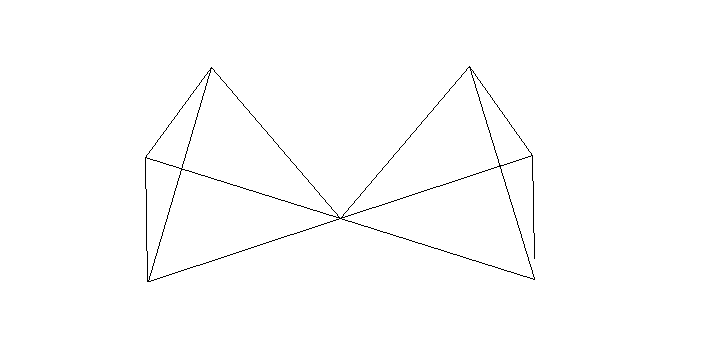
\includegraphics{tetratouch.png}
\caption{Two tetrahedra conjoined at a vertex.}
\label{fig:tt}
\end{figure}

\section{Future work}
\subsection{3-D}

We would also like to start investigating 3-dimensional constructs built from tetradrons. We can adjust our current code as much as we need to, and ultimately be able to evaluate Yamabe flow, as discussed by \cite{DrG}. While Yamabe flow is similar to Ricci flow, its value of $K_i$ is determined quite differently, involving not only the angles of the faces, but also the internal angles associated with them. We can also try and investigate how our code applies (if it does) to hyperbolic and spherical coordinates. 

\subsection{Circle packing expansions}

Circle packing is a very special way to characterize our side lengths. If we relax this criterium and let the circles overlap, we can introduce a second weight $\Phi$ that . We can then evaluate our side lengths as $$l_{ij} = \sqrt{r_i^2 + r_j^2 + 2r_ir_j\cos(\Phi(e_{ij}))}$$ With this more general interpretation, we can examine questions asked by Chow and Luo in \cite{chowluo}.  

\subsection{Hyperbolic/ spherical triangulations}

All this time we have focused on Euclidean coordinates. However, there are cased when triangulations may be better suited in other systems. In changing our format to hyperbolic and spherical coordinates, we would have to reevaluate each of our steps depending on the system. For example, in hyperbolic, the basic Ricci flow equation is $\displaystyle \frac{dr_i}{dt} = -K_i\sinh r_i$. Likewise, in spherical coordinates, $\displaystyle \sum{K_i} = 2\pi\chi - \mbox{Surface Area of surface}$, which can change over time. 

\section{Conclusions}
  We learned a lot of things along the way. At the beginning, we all had varying familiarities with college geometry; some of us hadn't touched the stuff since high school. But we are excited to see where Dr. Glickenstein's project is headed and we hope to remain a part of it in the months and years to come.\newline
  
  \noindent We would like to thank Dr. David Glickenstein for having us on this project, Dr. Robert Indik and the University of Arizona Math Department for their help and support, and the VIGRE foundation for making this possible. 
  
\newpage
\bibliography{Test1}  
\bibliographystyle{plain}

\newpage
\section*{Appendix}

\subsection*{Derivation of Eq.~(\ref{proof1})}
\maketitle
	
	We used the criteria $$f(\tilde{r_1},\tilde{r_2},\ldots,\tilde{r_n}) = \prod{\tilde{r_i}} = \prod{\alpha r_i} = \alpha^n\prod{r_i}= C$$ to constrain the values of radii. We take the derivative of $f$ with respect to $t$ and obtain
	\begin{eqnarray*}
	\frac{df}{dt} & = & n\alpha^{n-1}\frac{d\alpha}{dt}r_1r_2\ldots r_n + \alpha^n\frac{dr_1}{dt}r_2r_3\ldots r_n\\
								& + & \alpha^nr_1\frac{dr_2}{dt}r_3r_4\ldots r_n + \ldots + \alpha^nr_1r_2\ldots r_{n-1}\frac{dr_n}{dt}
	\end{eqnarray*}
	But since $\displaystyle \frac{dr_i}{dt} = -K_ir_i$ from Eq.~\ref{Riccif} we obtain
	\begin{eqnarray*}
	\frac{df}{dt} & = & \frac{n\alpha^{n}}{\alpha}\frac{d\alpha}{dt}r_1r_2\ldots r_n - K_1\alpha^nr_1r_2r_3\ldots r_n\\
								& - & K_2\alpha^nr_1r_2r_3r_4\ldots r_n - \ldots - K_n\alpha^nr_1r_2\ldots r_{n-1}r_n
	\end{eqnarray*}
	from which we can group terms and obtain
	\begin{eqnarray*}
	\frac{df}{dt} & = & (\alpha^nr_1r_2\ldots r_n)(\frac{n}{\alpha}\frac{d\alpha}{dt} - K_1 - K_2 - \ldots - K_n)\\
								& = & C(\frac{n}{\alpha}\frac{d\alpha}{dt} - K_1 - K_2 - \ldots - K_n)
	\end{eqnarray*}
	However, since the original product is a constant, we have $\displaystyle \frac{df}{dt} = 0.$ Thus we have $$\frac{n}{\alpha}\frac{d\alpha}{dt} - K_1 - K_2 - \ldots - K_n = 0$$
	Rearranging we have
$$\frac{1}{\alpha}\frac{d\alpha}{dt} = \frac{d(\log \alpha)}{dt} = \frac{K_1 + K_2 + \ldots + K_n}{n} = \overline{K}$$
	which we refer to as Eq.~(\ref{proof1})
  
  \subsection*{Remarks on Runge-Kutta method for solving Eq.~(\ref{Riccin})}
	\maketitle

The method used by Moreau in \cite{JPM} to solve a diffeential equation involves using a Runge-Kutta method. After investigating various methods to run our differential equation, we agreed that a Runge-Kutta format would be most beneficial for this type of problem. Even though it is more computationally complex than the simpler Euler's method, it makes up in its ability to converge and in its accuracy. According to $\cite{DiffEq}$ the error associated with using Runge-Kutta is on the order of $h^4$, whereas with a standard Euler approximation the error is simply of order $h$, with $h = dt$ being our step incremental. \newline

\noindent Based on our evaluations of radii and curvatures over time, it appears to converge exponentially for each vertex. However, as mentioned previously, performing flips on a triangulation may negate this and cause the system to go haywire. 

\begin{figure}[ht]
\centering
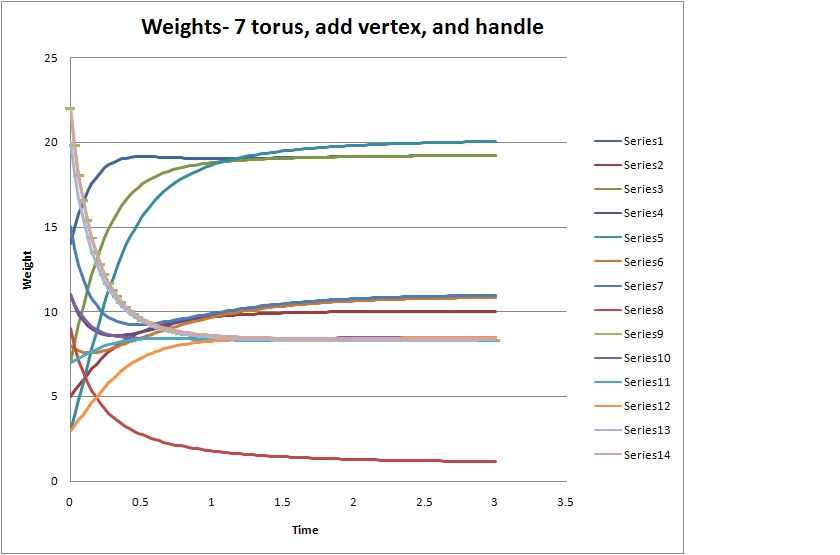
\includegraphics[scale = 0.9]{torus7addvaddhweights.png}
\end{figure}

\newpage
\subsection*{Code}
\begin{verbatim}void calcFlow(char* fileName, double dt ,double *initWeights,
				int numSteps, bool adjF)  
{
  int p = Triangulation::vertexTable.size(); // The number of vertices.
  double ta[p],tb[p],tc[p],td[p],z[p]; // Temporary arrays to hold data in.
  int    i,k; // ints used for "for loops".
  map<int, Vertex>::iterator vit;
  map<int, Vertex>::iterator vBegin = Triangulation::vertexTable.begin();
  map<int, Vertex>::iterator vEnd = Triangulation::vertexTable.end();
  double weights[p][numSteps];
  double curvatures[p][numSteps];
  
  ofstream results(fileName, ios_base::trunc);
  results.setf(ios_base::showpoint);
  double net = 0; // Net and prev hold the current and previous
  double prev;    //  net curvatures, repsectively.
   for (k=0; k<p; k++)
     z[k]=initWeights[k]; // z[k] holds the current weights.
   for (i=1; i<numSteps+1; i++) 
   {
    prev = net; // Set prev to net.
    net = 0;    // Reset net.
    
       for (k=0, vit = vBegin; k<p && vit != vEnd; k++, vit++)  
           // Set the weights of the Triangulation.
           vit->second.setWeight(z[k]);
       if(i == 1) // If first time through, use static method.
            prev = Triangulation::netCurvature();
       for (k=0, vit = vBegin; k<p && vit != vEnd; k++, vit++)  
       // First "for loop" in whole step calculates
       {                // everything manually, prints to file.
           weights[k][i - 1] = z[k];
           double curv = curvature(vit->second);
           curvatures[k][i - 1] = curv;
           net += curv;
           if(adjF) ta[k]= dt * ((-1) * curv 
                           * vit->second.getWeight() +
                           prev /  p
                           * vit->second.getWeight());
           else     ta[k] = dt * (-1) * curv 
                           * vit->second.getWeight();
       }
       for (k=0, vit = vBegin; k<p && vit != vEnd; k++, vit++)  
       // Set the new weights.
           vit->second.setWeight(z[k]+ta[k]/2);
       for (k=0, vit = vBegin; k<p && vit != vEnd; k++, vit++)  
       {
            if(adjF) tb[k]=dt*adjDiffEQ(vit->first, net);
            else     tb[k]=dt*stdDiffEQ(vit->first);
       }
       for (k=0, vit = vBegin; k<p && vit != vEnd; k++, vit++)  
       // Set the new weights.
           vit->second.setWeight(z[k]+tb[k]/2);
       for (k=0, vit = vBegin; k<p && vit != vEnd; k++, vit++)  
       {
            if(adjF) tc[k]=dt*adjDiffEQ(vit->first, net);
            else     tc[k]=dt*stdDiffEQ(vit->first);
       }
       for (k=0, vit = vBegin; k<p && vit != vEnd; k++, vit++)  
       // Set the new weights.
           vit->second.setWeight(z[k]+tc[k]);
       for (k=0, vit = vBegin; k<p && vit != vEnd; k++, vit++)  
       {
            if(adjF) td[k]=dt*adjDiffEQ(vit->first, net);
            else     td[k]=dt*stdDiffEQ(vit->first);
       }
       for (k=0; k<p; k++) // Adjust z[k] according to algorithm.
         z[k]=z[k]+(ta[k]+2*tb[k]+2*tc[k]+td[k])/6;
   }
   for(k=0, vit = vBegin; k<p && vit != vEnd; k++, vit++) 
   {  //Print results
      results << setprecision(6); 
      results << left << "Vertex: " << left << setw(4)<< vit->first;
      results << right << setw(3) << "Weight";
      results << right << setw(10) << "Curv";
      results << "\n------------------------------\n";
      for(int j = 0; j < numSteps; j++)
      {
              results << left <<  "Step " << setw(7) << (j + 1);
              results << left << setw(12) << weights[k][j];
              results << left << setw(12) << curvatures[k][j] << "\n";
      }
      results << "\n";
   }
   results.close();
}
\end{verbatim}
\begin{verbatim}
void flip(Edge e)
{
     //start out by naming every object that is local to the flip
     Face f1 = Triangulation::faceTable[(*(e.getLocalFaces()))[0]];
     Face f2 = Triangulation::faceTable[(*(e.getLocalFaces()))[1]];
     
     vector<int> sameAs;
     vector<int> diff;
     
     Vertex va1 = Triangulation::vertexTable[(*(e.getLocalVertices()))[0]];
     Vertex va2 = Triangulation::vertexTable[(*(e.getLocalVertices()))[1]];
          
     diff = listDifference(f1.getLocalVertices(), f2.getLocalVertices());
     if(diff.size() == 0)
     throw string("Invalid move, operation cancelled");
     Vertex vb1 = Triangulation::vertexTable[diff[0]];
     diff = listDifference(f2.getLocalVertices(), f1.getLocalVertices());
     Vertex vb2 = Triangulation::vertexTable[diff[0]];
     
     sameAs = listIntersection(va1.getLocalEdges(), vb1.getLocalEdges());
     Edge ea1 = Triangulation::edgeTable[sameAs[0]];
     sameAs = listIntersection(va2.getLocalEdges(), vb1.getLocalEdges());
     Edge eb1 = Triangulation::edgeTable[sameAs[0]];
     sameAs = listIntersection(va1.getLocalEdges(), vb2.getLocalEdges());
     Edge ea2 = Triangulation::edgeTable[sameAs[0]];
     sameAs = listIntersection(va2.getLocalEdges(), vb2.getLocalEdges());
     Edge eb2 = Triangulation::edgeTable[sameAs[0]];
     
     sameAs = listIntersection(f1.getLocalFaces(), ea1.getLocalFaces());
     Face fa1 = Triangulation::faceTable[sameAs[0]];
     sameAs = listIntersection(f1.getLocalFaces(), eb1.getLocalFaces());
     Face fb1 = Triangulation::faceTable[sameAs[0]];
     sameAs = listIntersection(f2.getLocalFaces(), ea2.getLocalFaces());
     Face fa2 = Triangulation::faceTable[sameAs[0]];
     sameAs = listIntersection(f2.getLocalFaces(), eb2.getLocalFaces());
     Face fb2 = Triangulation::faceTable[sameAs[0]];
     
     //removals
     Triangulation::vertexTable[(va1.getIndex())].removeVertex(va2.getIndex()); 
     Triangulation::vertexTable[(va2.getIndex())].removeVertex(va1.getIndex()); 
     Triangulation::vertexTable[(va1.getIndex())].removeEdge(e.getIndex()); 
     Triangulation::vertexTable[(va2.getIndex())].removeEdge(e.getIndex()); 
     Triangulation::vertexTable[(va1.getIndex())].removeFace(f2.getIndex()); 
     Triangulation::vertexTable[(va2.getIndex())].removeFace(f1.getIndex()); 
     Triangulation::edgeTable[(e.getIndex())].removeVertex(va1.getIndex()); 
     Triangulation::edgeTable[(e.getIndex())].removeVertex(va2.getIndex()); 
     for(int i = 0; i < e.getLocalEdges()->size(); i++)
     {
        Triangulation::edgeTable[(e.getIndex())]
        							.removeEdge((*(e.getLocalEdges()))[i]); 
     }
     for(int i = 0; i < va1.getLocalEdges()->size(); i ++)
     {
        Triangulation::edgeTable[(*(va1.getLocalEdges()))[i]]
        							.removeEdge(e.getIndex()); 
     }
     for(int i = 0; i < va2.getLocalEdges()->size(); i ++)
     {
        Triangulation::edgeTable[(*(va2.getLocalEdges()))[i]]
        							.removeEdge(e.getIndex());  
     }
     Triangulation::edgeTable[(eb1.getIndex())].removeFace(f1.getIndex()); 
     Triangulation::edgeTable[(ea2.getIndex())].removeFace(f2.getIndex()); 
     Triangulation::faceTable[(f1.getIndex())].removeVertex(va2.getIndex()); 
     Triangulation::faceTable[(f2.getIndex())].removeVertex(va1.getIndex()); 
     Triangulation::faceTable[(f1.getIndex())].removeEdge(eb1.getIndex()); 
     Triangulation::faceTable[(f2.getIndex())].removeEdge(ea2.getIndex()); 
     Triangulation::faceTable[(f1.getIndex())].removeFace(fb1.getIndex()); 
     Triangulation::faceTable[(fb1.getIndex())].removeFace(f1.getIndex()); 
     Triangulation::faceTable[(f2.getIndex())].removeFace(fa2.getIndex()); 
     Triangulation::faceTable[(fa2.getIndex())].removeFace(f2.getIndex()); 
     
     //additions
     Triangulation::vertexTable[(vb1.getIndex())].addVertex(vb2.getIndex()); 
     Triangulation::vertexTable[(vb2.getIndex())].addVertex(vb1.getIndex()); 
     Triangulation::vertexTable[(vb1.getIndex())].addEdge(e.getIndex()); 
     Triangulation::vertexTable[(vb2.getIndex())].addEdge(e.getIndex()); 
     Triangulation::vertexTable[(vb1.getIndex())].addFace(f2.getIndex()); 
     Triangulation::vertexTable[(vb2.getIndex())].addFace(f1.getIndex()); 
     Triangulation::edgeTable[(e.getIndex())].addVertex(vb1.getIndex()); 
     Triangulation::edgeTable[(e.getIndex())].addVertex(vb2.getIndex()); 
     for(int i = 0; i < vb1.getLocalEdges()->size(); i ++)
     {
             Triangulation::edgeTable[(e.getIndex())]
             						.addEdge((*(vb1.getLocalEdges()))[i]);
             						
             Triangulation::edgeTable[(*(vb1.getLocalEdges()))[i]]
             						.addEdge(e.getIndex()); 
     }
     for(int i = 0; i < vb2.getLocalEdges()->size(); i ++)
     {
             Triangulation::edgeTable[(e.getIndex())]
             						.addEdge((*(vb2.getLocalEdges()))[i]); 
             						
             Triangulation::edgeTable[(*(vb2.getLocalEdges()))[i]]
             						.addEdge(e.getIndex()); 
     }
     Triangulation::edgeTable[(ea2.getIndex())].addFace(f1.getIndex()); 
     Triangulation::edgeTable[(eb1.getIndex())].addFace(f2.getIndex()); 
     Triangulation::faceTable[(f1.getIndex())].addVertex(vb2.getIndex());
     Triangulation::faceTable[(f2.getIndex())].addVertex(vb1.getIndex());
     Triangulation::faceTable[(f1.getIndex())].addEdge(ea2.getIndex());
     Triangulation::faceTable[(f2.getIndex())].addEdge(eb1.getIndex());
     Triangulation::faceTable[(f1.getIndex())].addFace(fa2.getIndex());
     Triangulation::faceTable[(fa2.getIndex())].addFace(f1.getIndex());
     Triangulation::faceTable[(f2.getIndex())].addFace(fb1.getIndex());
     Triangulation::faceTable[(fb1.getIndex())].addFace(f2.getIndex());
     
}
\end{verbatim}
\section*{About the authors}

Alex Henniges is a junior double majoring in Math and Computer Science. Plus he's cool. He is the frontliner of the programming aspect of this research. \newline
  
\noindent Thomas Williams is a senior in Comprehensive Mathematics with a minor in Computer Science and a strong background in Math Education. He's cool, too. He made substantial contributions to the coding and development of this project.\newline
  
\noindent Mitch Wilson is a senior majoring in Applied Math and Mechanical Engineering. He's ok. He made the pretty pictures in this report, mostly using MATLAB. 

\end{document}